% ----------------- thesis chapters ----------------%
\chapter{Introduction}
\label{chap:intro}
%--------------------------------------------------%
\section{Overview of Compressive Sensing}
\label{sec: Chap_1_intro_CS}
In many problems of science and technology, one of the key tasks is to deduce quantities of interest from the measured high-dimensional data. For example, in image processing applications, one would like to reconstruct the signal (image) of interest from the observed measurements. In mathematical terms, the measurement vector  $\bm{y} \in \Re^{M \times 1}$ is related to the signal of interest $\bm{x} \in \Re^{N \times 1}$ via the sensing matrix $\bm{\Phi} \in \Re^{M \times N}$ as~\cite{Candes_CS, Candes_Comp_sampling}:
%
%----------------------------------------------------------------%
\begin{equation}
\label{eq:projections}
     \bm{y} = \bm{\Phi}\bm{x}
\end{equation}
%----------------------------------------------------------------%
%
%------------------%
Conventional techniques suggest that the number of measurements $M$, must be at least as large as the length of the underlying signal. This concept is related to the Nyquist-Shannon sampling theorem. However using compressed sensing (CS) techniques, it is possible to recover signals of length $N$ with the number of measurements being much smaller than $N$, provided the signal is sparse~\cite{Candes_Comp_sampling,CS_NS,Taocandes,Candes_Decoding,Romberg_imaging,Donoho}. In the CS framework, we can reconstruct the signal $\bm{x}$ from the measurement $\bm{y}$ assuming the relation in~\eqref{eq:projections} with $M \ll N$. This under-determined system has an infinite number of solutions for $\bm{x}$ and the sparsity constraint enables us to determine a unique solution. Compressed sensing is based on two fundamental principles:
%
A signal is said to be sparse if a large number of its values are zero or can be discarded without significant loss of information. Many real signals are compressible and can be approximated using sparse signals either directly or after application of an appropriate transform. If $\bm{x}$ is a real compressible signal, then it can be expressed as~\cite{Candes_CS, Candes_Comp_sampling}:
%------------------------%
\begin{equation}
\label{eq:transform_basis}
    \bm{x} = \sum_{i = 1}^{L} \theta_{i} \bm{\psi}_{i} + \bm{e} = \bm{\Psi}\bm{\theta} + \bm{e}
\end{equation}
%-----------------------%
where $\bm{\Psi} =[\bm{\psi}_1,\dots,\bm{\psi}_L] \in \Re^{N \times L}$ is the (sparsifying) transform basis, $\bm{\theta} \in \Re^{L\times 1}$ is the vector of sparse coefficients, $L$ is the number of the column vectors in the transform basis ($N \leq L$), and $\bm{e} \in \Re^{N}$ is the sparse encoding error (SEE). If $\bm{e} = \bm{0}$, then the signal $\bm{x}$ is said to be exactly sparse in $\bm{\Psi}$ with sparsity level $s=\|\bm{\theta}\|_{0}$, whereas if $\bm{e}$ is non-zero but has relatively low energy then $\bm{x}$ is said to be approximately $s$-sparse with $s=\|\bm{\theta}\|_{0}$. Here $\| \bm{\theta} \|_{0}$ denotes the number of non-zero elements in $\bm{\theta}$ and $\bm{0}$ represents a vector with all the elements being zero.
%
A well-approximated representation of the signal $\bm{x}$ requires appropriately designed projections. From~\eqref{eq:projections} and~\eqref{eq:transform_basis}, $\bm{y}=\bm{\Phi}\bm{\Psi}\bm{\theta} + \bm{\Phi}\bm{e}$, where $\bm{\Phi}$ is the sensing matrix, $\bm{\Phi} \bm{e}$ is the projected noise as a result of the SEE, and $\bm{D} = \bm{\Phi}\bm{\Psi}$ is the equivalent dictionary of the CS system. Let $\bm{D}  \in \Re^{M \times L}$  be a matrix with unit norm columns $\bm{d}_{1}, \bm{d}_{2},\dots,\bm{d}_{L}$, also known as atoms of the frame $\bm{D}$. Recovery of the underlying signal $\bm{x}$ requires the equivalent dictionary $\bm{D}$ to be as incoherent as possible. The coherence measure $\mu$ is given by:
%--------------------%
\begin{equation}
    \label{eq: mu_for_frame}
    \mu = \underset{1 \leq i\neq j \leq L}{\max}\lvert\langle \bm{d}_{i}, \bm{d}_{j}\rangle\rvert
\end{equation}
%----------------------%
which refers to the largest (or worst-case) absolute correlation between any two column vectors of $\bm{D}$~\cite{Sparse_union_bases,Donoho_optimal_sparse,Candes_CS}. A more generalised coherence metric is the cumulative coherence. Cumulative coherence measures the maximum total mutual coherence between a set of atoms and a collection of other atoms in the dictionary. It gives an indication of how far the dictionary is from an orthogonal basis. The cumulative coherence of a dictionary with normalized columns is defined as~\cite{Greed, BO_LI, shrinkage_sensing}:
%
\begin{equation}
    \label{eq: Cum_coherence}
    \mu_{1}(m) = \underset{\text{card}(\bm{\mathcal{P}}) = m}{\max}\; \left\{ \underset{j \in \bm{\mathcal{P}}}{\max}\left\{\underset{i \notin \bm{\mathcal{P}}}{\sum} \lvert\langle \bm{d}_{i},\bm{d}_{j} \rangle\rvert,  \right\}  \right\}
\end{equation}
%
where $\bm{\mathcal{P}} \subset \left[L\right]$ represents an identification number set of the column vectors in $\bm{D}$ and $1 \leq m \leq L-1$.
%and the $\text{card}(\bm{\mathcal{P}}) = m$. 
%Both i and j are the number of the column vectors in the dictionary $\bm{D}$. 
From~\eqref{eq: Cum_coherence}, we can show that $\mu_{1}(1) = \mu$ and that $\mu_{1}$ is a non-decreasing function of $m$.
%where $\mu$ is the maximum absolute inner product between the two column vectors of matrix $\bm{D}$. 
When the cumulative coherence of a dictionary increases slowly, we can say that the dictionary is quasi-incoherent~\cite{Greed}.

The Gram matrix of $\bm{D}$ is defined as $\bm{G} = \bm{D^{T}}\bm{D}$, which is a positive semidefinite and symmetric matrix with unit diagonal elements and rank $M$. The off-diagonal elements of $\bm{G}$ correspond to the inner product of two distinct atoms of $\bm{D}$. To recover the signal from under-sampled measurements, CS requires sparsity of $\bm{x}$ and incoherence of $\bm{D}$. Assuming $\bm{y}$ and $\bm{D}$ are known, $\bm{x}$ can be obtained by solving~\cite{Atomic_BP, Greed_OMP, OMP_new}:
%--------------------%
\begin{equation}
    \label{eq:L0_reconstruction}
    \underset{\bm{\theta}}{\min}\, \| \bm{y} - \bm{D}\bm{\theta}\|_{2}  \quad \text{s.t.} \quad \|\bm{\theta}\|_{0} \leq s % = % \bm{\Phi}\bm{\Psi}\bm{\theta}
\end{equation}
%---------------------%
which is NP-hard. Greedy algorithms, such as orthogonal matching pursuit (OMP)~\cite{Atomic_BP, Greed_OMP, Tropp}, matching pursuit (MP)~\cite{Mallat}, generalized OMP~\cite{Jian}, and others~\cite{chen_recovery} can be employed to solve~\eqref{eq:L0_reconstruction} for $\bm{\theta}$ under certain conditions (with theoretical guarantees) and recover $\bm{x}$. For a fixed transform basis $\bm{\Psi}$, sensing matrix is a key determinant in the performance of the recovery algorithms, both convex relaxation-based and greedy algorithms. Optimized sensing matrix can achieve improved signal recovery performance using under-sampled measurements~\cite{Elad}. 

If $\bm{y}$ is captured using the frame $\bm{D}$, the signal $\bm{x}$ with sparsity $s$ can be recovered by solving~\eqref{eq:L0_reconstruction}, provided the following constraint is satisfied~\cite{Greed}:
%-----------------------%
\begin{equation}
    \label{eq:sparse_bound}
    s < \frac{1}{2}\left(1 + \frac{1}{\mu}\right)
\end{equation}
%-----------------------%
The largest absolute value of the pairwise correlation is lower bounded by the Welch bound (WB) ($\mu_{W}$)~\cite{welch}, and when the signal dimension $N \leq M^{2}$, is given by:
%---------------------%
\begin{equation}
    \label{eq:welch}
    \mu \geq \mu_{W} \triangleq \sqrt{\frac{(L-M)}{M(L-1)}}
\end{equation}
%---------------------%
The $t$-averaged mutual coherence $\mu_{t}$~\cite{Elad}, for a given coherence threshold $t$, is an alternative metric for evaluating recovery performance achieved using a projection matrix and is given by:
%-------------------%
\begin{equation}
    \label{eq:mu_t}
    \mu_{t} = \frac{\underset{1 \leq i\neq j \leq L}{\sum}\left(\lvert \bm{G}_{ij}\rvert\geq t\right)\cdot\lvert \bm{G}_{ij}\rvert}{\underset{1\leq i\neq j\leq L}{\sum}\left(\lvert \bm{G}_{ij}\rvert\geq t\right)}
\end{equation}
%---------------------%
These coherence measures will be used as the performance metrics for evaluating the efficacy of the optimized sensing matrix. Restricted isometry property (RIP) and spark of the projection matrix can be effective in evaluating the effect of optimized projections~\cite{Taocandes},~\cite{Donoho},~\cite{Candes_CS},~\cite{Near_optimal}. The restricted isometry constant (RIC) $\delta_{s} \in \left(0,1\right)$ is the smallest value of $\delta$ that satisfies~\cite{Donoho_optimal_sparse}:
%------------------%
\begin{equation}
    \label{RIP}
    (1-\delta)\|\bm{\theta}\|_{2}^{2} \leq \|\bm{\Phi}\bm{\Psi}\bm{\theta}\|_{2}^{2} \leq (1+\delta) \|\bm{\theta}\|_{2}^{2}
\end{equation}
%------------------%
where $\bm{\theta} \in \Re^{L\times 1}$ is an arbitrary $s$-sparse signal. Spark of a matrix is defined as the smallest number of linearly dependent columns. The sensing matrix plays two key roles. Firstly, it determines how close the sparsest solution obtained using~\eqref{eq:L0_reconstruction} would be to the original signal. For a noise-free CS system, the RIC $\delta_{2s} < 1$ guarantees that the solution of~\eqref{eq:L0_reconstruction} will equal the original signal~\cite{Candes_Decoding}. The condition for the greedy algorithm to perfectly identify the sparse coefficients %successful recovery 
is expressed as $\mu < \frac{1}{2s-1}$, or $\mu(s)+\mu(s-1) < 1$~\cite{Greed}. Secondly, sensing matrix affects the recovery performance. With RIC $\delta_{s} < \frac{\sqrt{4s+1}-1}{2s}$ ensures the recovery of a sparse signal approximation using OMP when there is no measurement noise~\cite{RIP_chang}.

\subsection{Closer Look at Frame Theory}
\label{subsec: Chap1_Frame}
%
A frame $\bm{D}$ in a real or complex $M$-dimensional Hilbert space can be represented as a sequence of $L \left(\geq M\right)$ basis vectors $\{\bm{d}_{k}\}_{k = 1}^{L}$, $\bm{d}_{k} \in \mathcal{H}^{M}$, satisfying the Parseval's condition ~\cite{Frame_welch,Foucart}:
%-----------------------%
\begin{equation}
\label{eq:parseval}
 \alpha\|\bm{v}\|^{2}_{2}\leq \|\bm{D}^{T}\bm{v}\|_{2}^{2} \leq\beta\|\bm{v}\|^{2}_{2},\quad \forall\bm{v}\in\mathcal{H}^{M}
\end{equation}
%-----------------------%
where $\alpha$ and $\beta$ are positive constants. If all the frame vectors have unit $\ell_{2}$-norm i.e., $\|\bm{d}_{k}\|_{2} = 1 \, \forall k$, the frame is known as unit norm frame (UNF). A frame is an equiangular frame if there exists a constant $c \in (0,1)$ such that $\lvert\langle \bm{d}_{i},\bm{d}_{j}\rangle\rvert = c, \forall\, i \neq j$.
A frame with the smallest maximum correlation among all UNFs $\in \Re^{M \times L}$ in a finite dimension is said to be a Grassmannian frame~\cite{STROHMER_frame}.
The measure of over-completeness or redundancy of a frame $\bm{D}$ is given by $\rho = L/M$~\cite{STROHMER_frame}. If $\alpha =\beta$, then $\bm{D}$ is said to be an $\alpha$-tight frame which satisfies the relation $\sum_{k=1}^{L} \|\bm{d}_{k}\|_{2}^{2} = \alpha M$. In CS, Welch bound for mutual coherence can be achieved with an equiangular tight frame (ETF) as it has low averaged mutual coherence which is essential for the minimal dependency property. An equiangular tight frame is a unit-norm tight frame (UNTF) in which each pair of column vectors has the same absolute inner product~\cite{STROHMER_frame}. 

%%% -------------------------------------%%
\section{Overview of Feature Extraction}
\label{sec: Chap_1_feature Extraction overview}
%
Visual recognition such as face, object, and scene recognition have been a subject of extensive research in computer vision. Extensive literature exists on feature extraction and learning models for recognition. However, in real world applications, captured images show multitude variations such as varying lighting, poses, facial expressions, structural properties, and occlusions. Such variations can be caused by the changes in camera, object viewpoint, illumination conditions, environment where pictures are captured, etc. These variations are the major challenges for real world pattern recognition and computer vision applications. Hence, the learning models tend to require large amounts of data and features to capture the variations in the data. Many of these features are correlated or redundant, and this is where feature extraction algorithms play an important role.

Feature extraction aims to identify an optimal set of features from a data set by creating new features from the existing ones. Features are the parts or patterns of an object in an image that help to recognize it. For e.g., a rectangle has $4$ corners and $4$ edges, which can be called features of the rectangle, and they help us identify it’s a rectangle. Features include characterstics like corners, edges, regions of interest points, ridges, eyes, nose, ears etc represented by a set of pixels in images. An important attribute of large data sets is the large number of features that require a lot of computing resources for processing. The large data is suspected to be redundant (e.g. the same measurement in both feet and centimeters, or the repetitiveness of images presented as pixels), which can be transformed into a reduced set of features (also named a feature vector). %Feature extraction can effectively build these derived values (feature vectors) intended to be informative and non-redundant
%reduce the amount of data for processing, while still %\textcolor{red}{accurately and completely}
%representing the original data set. 
The feature vectors are expected to contain the relevant information from the input data, so that the desired object in the image can be identified by using this reduced representation instead of the complete initial data.
%The main goal is to identify fewer features that can adequately capture the \textcolor{blue}{relevant information}. The selected features are expected to contain the relevant information from the input data, so that the desired task can be performed by using this reduced representation instead of the complete initial data.  %However, when we reduce the dimensionality of a data set, we lose some of the \textcolor{red}{information} depending on the number of features retained.
%, but such data usually comprise of noise and/or redundant information. 
The following are the advantages of feature extraction.
%
\begin{itemize}
    \item Reduced dimensionality of data implies less training time and fewer computational resources.  
    \item Feature extraction avoids the problem of overfitting. For a data set with too many features, the models become complex and tend to overfit. Feature extraction can transform the data to an optimal set of features with the relevant information being retained. 
    \item Feature extraction helps in data visualization. With reduced dimensionality of the high dimensional data, we can easily visualize the data.
    \item Feature extraction takes advantage of the correlation among the data samples and can combine the highly correlated samples together and the uncorrelated samples as well. This will help in preserving the underlying intrinsic structure of the data samples.
    \item Feature extraction retains only the significant features and removes the redundant ones, and hence helps in removing noise from the data. This will improve the overall performance of the model.
\end{itemize}
%%=============================================================%
\section{Main Hypothesis and Contributions}
\label{sec: chap1_hypothesis}
%
The research hypothesis of this thesis is based on computer vision and pattern recognition applications related to image reconstruction and image classification tasks. The research work focuses on two broad categories of research problems: compressed sensing based sensing matrix design and feature extraction based dimensionality reduction for image reconstruction and image classification applications. The main hypothesis of this thesis is to design an incoherent and robust sensing matrix and the development of feature extraction models for image classification. As discussed in Sections~\ref{sec: Chap_1_intro_CS} and~\ref{sec: Chap_1_feature Extraction overview}, representing high-dimensional data so as to extract its key properties can significantly affect the performance of pattern recognition and computer vision based applications while reducing the memory requirements.

For CS-based sensing matrix design, it is essential to extract significant data samples from the high-dimensional data using sparsity for image reconstruction applications. The challenge is to optimize an incoherent sensing matrix with respect to an equiangular tight frame. Further, for robust image reconstruction, an incoherent and robust sensing matrix design is required to extract the significant information even in the presence of noisy. Hence, the first contribution is the reconstruction of the high-dimensional sparse signal from its low-dimensional linear projection measurements. To this end, the thesis proposes to optimize the sensing matrix to extract sufficient measurements for recovery.

%Additionally, from Section~\ref{sec: Chap_1_feature Extraction overview}, we can say that 
The high dimensional data used in computer vision and pattern recognition tasks usually contains significant redundancy which can result in redundant features and increased computational complexity and memory requirements, as well as the possibility of overfitting. This can weaken the structural relationship between the samples degrading the overall performance. Thus, the challenge is to obtain a compact low-dimensional representation and features with good generalization capability and discriminative ability for applications such as face recognition, object classification, and scene classification.

In this thesis, one of the major hypotheses is to develop feature extraction models to extract significant and discriminative low-dimensional features. The first challenge is to explore the underlying global and local structure of the high-dimensional data while preserving the discriminative ability of the optimized low-dimensional features. Next challenge is to develop a feature extraction model to address the problems of insufficient inter-class margin and loss of the manifold structure of the data. The overall aim is to extract a set of low-dimensional features while preserving the neighborhood affinity among the data samples resulting in improved performance in pattern recognition applications. Hence, this thesis contributes to the design of framework for mapping high-dimensional data to low-dimensional compact features while preserving the underlying structure. In the next chapter, we present a literature review followed by a discussion of the motivation and models for the proposed frameworks.
%==============================================================%
%===================================================%
\section{Summary of Contributions}
\label{sec: Chap1_contri}
The main contributions of this thesis are summarized as follows:

\begin{itemize}
    \item We propose a sensing matrix design method that can account for the sparse encoding error while extracting significant measurements from the high-dimensional data.
    \item We propose a local adaptive structure that preserves the intra-class similarity among the neighboring transformed features for representation-based feature extraction.
    \item We propose a relaxed target regression method integrated with a classwise mean constraint for pattern recognition applications.
    \item We integrate the robust $\ell_{2,1}$-norm in the sensing matrix design and feature extraction algorithms for extracting measurements and features from corrupted data samples.
\end{itemize}
%%=============================================================%%
\section{Thesis Outline}
%
The work presented in this thesis is focused on two broad areas: incoherent and robust sensing matrix design, and feature extraction algorithms. An overview of the thesis organization is provided below and illustrated in Fig.~\ref{fig: Organization}.
%
\begin{figure}
\centering
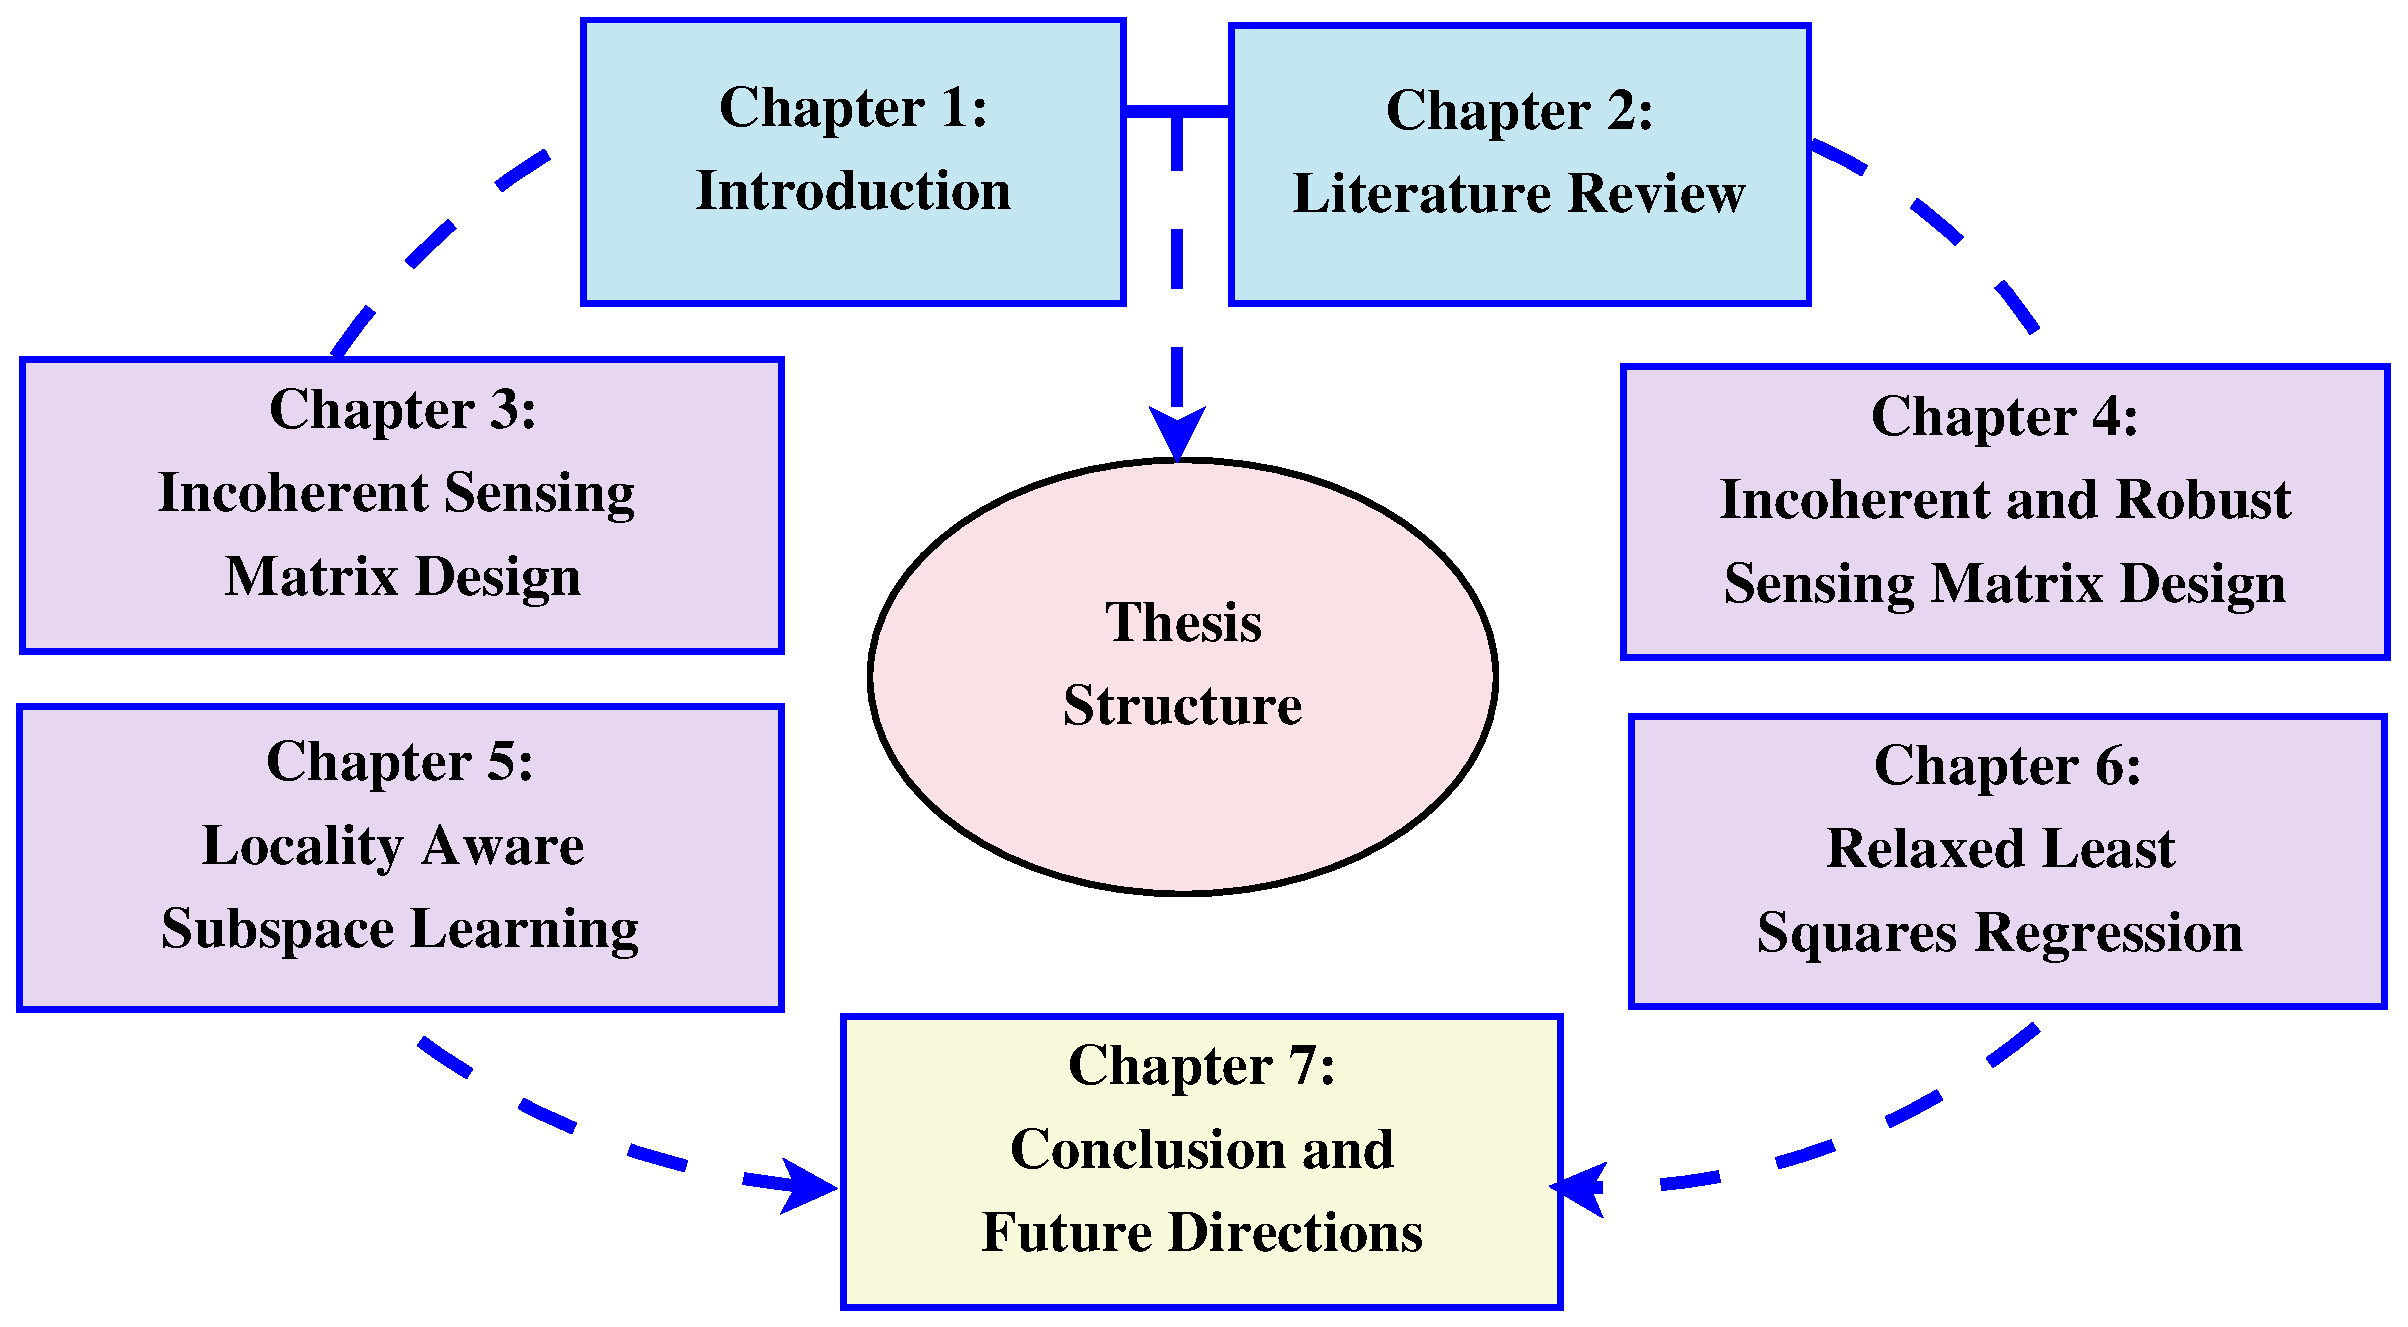
\includegraphics[keepaspectratio,width=1.0\textwidth,trim=0 0 0 0,clip]{Thesis_Org.eps}
\caption{Illustration of thesis organization.}
\label{fig: Organization}
\end{figure} 
%
\begin{enumerate}
\item Chapter 1 provides background information on the concepts of compressed sensing and dimensionality reduction.
\item Chapter 2 gives an overview of sensing matrix design, feature extraction methods, state-of-the-art algorithms, and the research challenges that will be addressed in this thesis.
\item Chapter 3 describes the proposed sensing matrix design to construct an incoherent sensing matrix and a corresponding ETF for image reconstruction.
\item Chapter 4 presents an incoherent and robust sensing matrix design method. The algorithm constructs a robust sensing matrix with an additional sensing matrix energy constraint and an adaptive weighted penalty.
\item Chapter 5 presents a locality-aware subspace learning model. The algorithm jointly optimizes the projection matrix and classification error to extract compact and low-dimensional features. 
\item Chapter 6 presents regression-based feature extraction algorithms. First, a low-rank double relaxation based regression algorithm is proposed for image classification. Further, a twin relaxed method is presented based on the relaxed target and intra-class similarity of the original data set.
\item Chapter 7 presents the concluding remarks and future research directions based on the frameworks proposed in this thesis.
\end{enumerate}

